\documentclass[12pt,a4paper]{report}
%\documentclass[12pt, twoside,openright]{report}
\usepackage[]{graphicx}
%\usepackage{fontspec}
%\setmainfont{Code2000}
%\usepackage{,epsfig}
\usepackage[centertags]{amsmath}
\usepackage{epstopdf,amsfonts,epsfig,cite,array,multirow,graphicx,amsmath,amsthm,ltablex,tabularx,setspace,arydshln,amssymb,multirow,enumerate}
%%%%%%% Inline listing package
%\usepackage[inline]{enumitem}
\DeclareMathOperator{\arccot}{arccot}
\DeclareMathOperator{\sinc}{sinc}
%\usepackage{marvosym}
%\usepackage{moderncvcompatibility}
\usepackage{geometry}
\geometry{tmargin=20mm,bmargin=20mm,lmargin=30mm,rmargin=25mm}
%\usepackage[cmex10]{amsmath}
\newcommand{\matr}[1]{\mathbf{#1}}

%%%%%%%%%%%% Run this package final time or if any error %%%%%%%%%
%\usepackage{fancyhdr}
\usepackage[titletoc]{appendix}
\usepackage[usenames,dvipsnames]{xcolor}
\usepackage{graphics}
\usepackage{cite}
\usepackage{amsmath}
\usepackage{amssymb}
\usepackage{amsfonts}
\usepackage{tikz}
\usepackage{setspace}
\usepackage{color}
\usepackage{relsize}
\usepackage{bigints}
\usetikzlibrary{shapes,arrows,fit,calc,positioning}
\usetikzlibrary{decorations.shapes}
\definecolor{colorgreen}{rgb}{0.2,0.5,0.3}
\definecolor{colorblue}{rgb}{0,0,0}
\usetikzlibrary{decorations.pathmorphing}
\usepackage{subfigure}
%\usepackage{hyperref}
\usepackage{ellipsis}
\usetikzlibrary{calc}
\usetikzlibrary{decorations.pathreplacing,decorations.markings,shapes.geometric}
\tikzset{naming/.style={align=center,font=\small}}
\tikzset{antenna/.style={colorblue, thick,insert path={-- coordinate (ant#1) ++(0,0.2) -- +(135:0.2) + (0,0) -- +(45:0.2)}}}
\tikzset{station/.style={naming,draw,shape=dart, thick,colorblue,shape border rotate=90, minimum width=15mm, minimum height=15mm,outer sep=0pt,inner sep=3pt}}
\tikzset{stationnew/.style={naming,draw,shape=dart, thick,colorblue,shape border rotate=90, minimum width=20mm, minimum height=20mm,outer sep=0pt,inner sep=3pt}}
%\tikzset{mobile/.style={naming,draw,shape=rectangle,minimum width=15mm,minimum height=7.5mm, outer sep=0pt,inner sep=3pt}}
\tikzset{mobile/.style={naming,draw,shape=rectangle,fill=olive!40,minimum width=3mm,minimum height=3mm, outer sep=0pt,inner sep=3pt}}
\tikzset{radiation/.style={{decorate,decoration={expanding waves,angle=90,segment length=4pt}}}}
\tikzset{
  double arrow/.style args={#1 colored by #2 and #3}{
    -stealth,line width=#1,#2, % first arrow
    postaction={draw,-stealth,#3,line width=(#1)/3,
                shorten <=(#1)/3,shorten >=2*(#1)/3}, % second arrow
  }
}

\tikzset{
  double dasharrow/.style args={#1 colored by #2 and #3}{
    -stealth,dashed,line width=#1,#2, % first arrow
    postaction={draw,-stealth,#3,line width=(#1)/3,
                shorten <=(#1)/3,shorten >=2*(#1)/3}, % second arrow
  }
}



\newcommand{\UE}[1]{%
\begin{tikzpicture}[every node/.append style={rectangle,minimum width=0pt}]
\node[mobile] (box) {#1};

\draw ([xshift=.25cm] box.south west)
      ([xshift=-.25cm]box.south east);

%\fill ([xshift=.25cm] box.south west) circle (1pt)
%      ([xshift=-.25cm]box.south east) circle (1pt);

\draw (box.north) [antenna=1];
\end{tikzpicture}
}



\newcommand{\BS}[1]{%
\begin{tikzpicture}
\node[station] (base) {#1};

%\draw[line join=bevel] (base.110) -- (base.70) -- (base.north west) -- (base.north east) -- cycle;
\draw[line join=bevel,colorblue] (base.100) -- (base.80) -- (base.110) -- (base.70) -- (base.north west) -- (base.north east);
\draw[line join=bevel,colorblue] (base.100) -- (base.70) (base.110) -- (base.north east);

% original yshift=.8pt
\draw[line cap=rect] ([yshift=0pt]base.north) [antenna=1];
\end{tikzpicture}
}

\newcommand{\BSnew}[1]{
	\begin{tikzpicture}[scale=2.0]
	\node[stationnew] (base) {#1};
	
	\draw[line join=bevel] (base.110) -- (base.70) -- (base.north west) -- (base.north east) -- cycle;
	\draw[line join=bevel,colorblue] (base.100) -- (base.80) -- (base.110) -- (base.70) -- (base.north west) -- (base.north east);
	\draw[line join=bevel,colorblue] (base.100) -- (base.70) (base.110) -- (base.north east);
	
	% original yshift=.8pt
	\draw[line cap=rect] ([yshift=0pt]base.north) [antenna=1];
	\end{tikzpicture}
}

\newcommand{\RELAY}[1]{%
\begin{tikzpicture}[scale=0.2]
%\node[] (naming) {#1};
            \draw[thick,colorblue] (0,0) -- (1,4);% left line
            \draw[thick,colorblue] (3,0) -- (2,4);% right line
            \draw[semithick,colorblue] (0,0) arc (180:0:1.5 and -0.5) node[above, midway]{#1};
            \node[inner sep=4pt,colorblue] (circ) at (1.5,5.5) {};
            \draw[semithick,colorblue] (1.5,5.5) circle(8pt);
            \draw[semithick,colorblue] (1.5,5.5cm-8pt) -- (1.5,4);
            \draw[semithick,colorblue] (1.5,4) ellipse (0.5 and 0.166);
            \draw[semithick,radiation,decoration={angle=45}] (1.5cm+8pt,5.5) -- +(0:2);
            \draw[semithick,radiation,decoration={angle=45}] (1.5cm-8pt,5.5) -- +(180:2);
            %\fill[color = Aquamarine!80](0,0)--(1,4) -- (2,4)--(3,0)--cycle ;


\end{tikzpicture}
}

\newcommand{\RELAYnew}[1]{%
	\begin{tikzpicture}[scale=0.25]
	%\node[] (naming) {#1};
	\draw[thick,colorblue] (0,0) -- (1,4);% left line
	\draw[thick,colorblue] (3,0) -- (2,4);% right line
	\draw[semithick,colorblue] (0,0) arc (180:0:1.5 and -0.5) node[above, midway]{#1};
	\node[inner sep=4pt,colorblue] (circ) at (1.5,5.5) {};
	\draw[semithick,colorblue] (1.5,5.5) circle(8pt);
	\draw[semithick,colorblue] (1.5,5.5cm-8pt) -- (1.5,4);
	\draw[semithick,colorblue] (1.5,4) ellipse (0.5 and 0.166);
	\draw[semithick,radiation,decoration={angle=45}] (1.5cm+8pt,5.5) -- +(0:2);
	\draw[semithick,radiation,decoration={angle=45}] (1.5cm-8pt,5.5) -- +(180:2);
	%\fill[color = Aquamarine!80](0,0)--(1,4) -- (2,4)--(3,0)--cycle ;
	
	
	\end{tikzpicture}
}

\newcommand{\MBS}[1]{%
\begin{tikzpicture}
\node[stationnew] (base) {#1};

%\draw[line join=bevel] (base.110) -- (base.70) -- (base.north west) -- (base.north east) -- cycle;
\draw[line join=bevel,colorblue] (base.100) -- (base.80) -- (base.110) -- (base.70) -- (base.north west) -- (base.north east);
\draw[line join=bevel,colorblue] (base.100) -- (base.70) (base.110) -- (base.north east);

% original yshift=.8pt
%\draw[line cap=rect] ([xshift=.5cm,yshift=.3pt] base.north) [antenna=1];
%\draw[line cap=rect] ([yshift=.3pt]ant1 |- base.north) -- node[above,shape=rectangle,inner ysep=+.3333em]{\dots} ([xshift=-.5cm,yshift=.3pt]base.north) [antenna=2];
\draw[line cap=rect] ([xshift=-.1768cm,yshift=.6pt]base.north -| base.right tail) [antenna=1];

\draw[line cap=rect] ([yshift=.6pt]ant1 |- base.north) -- node[above,shape=rectangle,inner ysep=+.3333em]{\dots} ([xshift=.1768cm,yshift=.6pt]base.north -| base.left tail) [antenna=2];

\draw[line cap=rect] ([yshift=.6pt]ant1 |- base.north) -- node[above,shape=rectangle,inner ysep=+.3333em,]{\dots} ([xshift=.1768cm,yshift=.6pt]base.north -| base.left tail) [antenna=3];
%\draw[line cap=rect] ([yshift=.3pt]ant1 |- base.north) -- ([xshift=-.5cm,yshift=.3pt]base.north) [antenna=2];
%\node at ($(ant1)!0.5!(ant2)$) {\dots};
\end{tikzpicture}
}


\newcommand{\MOBILE}[1]{%
\begin{tikzpicture}[scale=0.25]
\begin{scope}[line join=round,looseness=0.25, line cap=round]
\begin{scope}
\clip [preaction={left color=blue!10, right color=blue!30}]
  (1/2,-1) to [bend left] (0,10)
  to [bend left] ++(1,1) -- ++(0,2)
  arc (180:0:3/4 and 1/2) -- ++(0,-2)
  to [bend left]  ++(5,-2) coordinate (A) to [bend left] ++(-1/2,-11)
  to [bend left] ++(-1,-1) to [bend left] cycle;
%
\path [left color=blue!30, right color=blue!50]
  (A) to [bend left] ++(0,-11) to[bend left] ++(-3/2,-2)
  -- ++(0,12);
%
\path [fill=blue!20, draw=white, line width=0.25cm]
  (0,10) to [bend left] ++(1,1) -- ++(0,2)
  arc (180:0:3/4 and 1/2) -- ++(0,-2)
  to [bend left]  (A) to [bend left] ++(-3/2,-5/4)
  to [bend right] cycle;
%
\draw [line width=0.25cm, fill=white]
  (9/8,21/2) arc (180:360:5/8 and 3/8) --
  ++(0,2.5) arc (0:180:5/8 and 3/8) -- cycle;
%
\draw [line width=0.25cm, fill=white]
  (9/8,13) arc (180:360:5/8 and 3/8);
%
\fill [white, shift=(225:0.5)]
  (1,17/2) to [bend left] ++(4,-7/4)
  to [bend left] ++(0,-7/2) to [bend left] ++(-4, 6/4)
  to [bend left] cycle;
%
\fill [black, shift=(225:0.25)]
  (1,17/2) to [bend left] ++(4,-7/4)
  to [bend left] ++(0,-7/2) to [bend left] ++(-4, 6/4)
  to [bend left] cycle;
%
\shade [inner color=white, outer color=cyan!20]
  (1,17/2) to [bend left] ++(4,-7/4)
  to [bend left] ++(0,-7/2) to [bend left] ++(-4, 6/4)
  to [bend left] cycle;
\draw [line width=0.25cm, shorten <=-0.5cm, shorten >=-0.5cm]
  (1,17/2) to [bend left] ++(4,-7/4)
  to [bend left] ++(0,-7/2);
%
\foreach \i in {1,2,3}
  \foreach \j in {1,2,3}
     \draw [line width=0.125cm, top color=gray,
       bottom color=white, yslant=-3/8, rounded corners=1cm/8]
         (\i*3/2-1/2,-\j+4) rectangle ++(1,3/4);
%
\draw [line width=0.125cm, top color=gray, bottom color=white, yslant=-3/8]
  (3,0) ellipse [x radius=1/2, y radius=1/3];
%
\draw [line width=0.125cm, top color=gray, bottom color=white, yslant=-3/8]
  (3,19/2) ellipse [x radius=1, y radius=1/4];
\end{scope}
\draw [line width=0.5cm]
  (1/2,-1) to [bend left] (0,10)
  to [bend left] ++(1,1) -- ++(0,2)
  arc (180:0:3/4 and 1/2) -- ++(0,-2)
  to [bend left]  ++(5,-2) to [bend left] ++(-1/2,-11)
  to [bend left] ++(-1,-1) to [bend left] cycle;
\end{scope}%

\end{tikzpicture}
}

\usepackage[acronym,nomain]{glossaries}
\usepackage{amsthm}
\usepackage{amssymb}
\usepackage{graphicx,subfigure}
%\usepackage[center]{caption}
\usepackage{amsmath}
\usepackage{graphicx}
%\usepackage[chapter]{algorithm}
\usepackage{algpseudocode}

%\usepackage{algorithm}
%\usepackage{algorithmic}

\usepackage{dcolumn}
\usepackage{bigints}
\usepackage{psfig}

\usepackage{cite}
%\usepackage{subcaption}
 \usepackage{notoccite}
\usepackage{float}
%\usepackage{subfig}
%\usepackage{graphicx}
\usepackage{caption}
%\usepackage{longtable}

%\usepackage{color}   %May be necessary if you want to color links
%\usepackage{hyperref}
%\hypersetup{
%	breaklinks=true,
%    colorlinks=true, %set true if you want colored links
%    linktoc=all,     %set to all if you want both sections and subsections linked
%    linkcolor=black,  %choose some color if you want links to stand out
%}

\usepackage{hyperref}
\hypersetup{breaklinks=true, colorlinks=true, linkcolor=black, citecolor=black}

\hypersetup{urlcolor=black}


\DeclareMathOperator*{\argmin}{arg\;min}
\DeclareMathOperator*{\argmax}{arg\;max}
\newcounter{MYtempeqncnt}
%\usepackage{url}
%\usepackage{bbm}
%\usepackage{eufrak}
%%%%%%%%%%%%%
\newtheorem{theorem}{Theorem}[chapter]
\newtheorem{proposition}{Proposition}[chapter]
\newtheorem{lemma}{Lemma}[chapter]
\newtheorem{definition}{Definition}[chapter]


\newcommand\blfootnote[1]{%
\begingroup
\renewcommand\thefootnote{}\footnote{#1}%
\addtocounter{footnote}{-1}%
\endgroup
}




% \pagestyle{fancy}
% \renewcommand{\sectionmark}[1]{\markright{\thesection\ #1}}
% \fancyhf{}
 %\lhead{\fancyplain{}{\rightmark }}
 %\cfoot{\fancyplain{}{\thepage}}

%\doublespacing
%
%

%
%
\setlength{\parindent}{1em}
\setlength{\parskip}{1.25em}
\renewcommand{\baselinestretch}{1.35}

\newtheorem{prop}{Proposition}
%-------------------------------------------------------------------
%\renewcommand{\contentsname}{Table of Contents}

%\makeatother
\usepackage{fancyhdr}
\usepackage{lipsum}% just to generate text for the example
%%%%%%%%%% To rename Table of Contents
\renewcommand{\contentsname}{Contents}
%%%%%%%%%%
%\flushbottom
%--------------------------------------------------------------------------
\raggedbottom                               % (Remove Unnecessary space b/w paragraphs)
%--------------------------------------------------------------------------
\begin{document}

\pagenumbering{roman}
% --------- Title and abstract etc the front matter -----------
% TITLE PAGE
\begin{titlepage}
\thispagestyle{empty}
\begin{center}
{\Large  \bf A 16-way Time-Interleaved SAR ADC Design for SerDes Links at 16 Gbps}
\end{center}
% \vspace{-2.5em}
% \begin{center}
%  \textbf{COMMUNICATION SYSTEMS OVER FADING CHANNELS}
% \end{center}
 \vspace{2em}
\begin{center}
 \textbf{\textit{Report submitted to the}}
\end{center}
 \vspace{-3em}
\begin{center}
 \textbf{\textit{Indian Institute of Technology  Bhubaneswar}} 
\end{center}
 \vspace{-3em}
\begin{center}
 \textbf{\textit{For mid-semester review}} 
\end{center}
 \vspace{-1em}
\begin{center}
 \textbf{\textit{of}}
\end{center}
 \vspace{-1em}
\begin{center}
 \textbf{\large Master of Technology Project Work}
\end{center}
 \vspace{-1em}
\begin{center}
 \textbf{\textit{by}}
\end{center}
 \vspace{-1em}
\begin{center}
 \large{\textbf{K ADITYA SAI}}
\end{center}
 \vspace{-1em}
\begin{center}
 Under the guidance of
\end{center}
 \vspace{-1em}
\begin{center}
 \textbf{Dr Nijwm Wary}
\end{center}
 \vspace{-1em}
\begin{center}

\includegraphics[scale=0.3]{iitbbs}
\end{center}
 \vspace{-1em}
\begin{center}
 \textbf{\small SCHOOL OF ELECTRICAL SCIENCES}
\end{center}
 \vspace{-3em}
\begin{center}
 \textbf{\small INDIAN INSTITUTE OF TECHNOLOGY BHUBANESWAR} 
\end{center}
 \vspace{-3em}
\begin{center}
 \textbf{September 2022}
\end{center}
 \vspace{-3em}
\begin{center}
 \copyright 2022 K Aditya Sai. All rights reserved.
\end{center}
%\newpage
%\thispagestyle{empty}
\cleardoublepage

\end{titlepage}


\newpage
%%%%%%%%%%
\pagenumbering{roman}
 %\addcontentsline{toc}{chapter}{Certification of Approval}
%% Page 3 : Approval of the DSC
%\thispagestyle{empty}
%\begin{center}
%	\textbf{\Large APPROVAL OF THE VIVA-VOCE BOARD}
%\end{center}
%\begin{flushright}
%	30/09/2022
%\end{flushright}
%~~~Certified that the thesis entitled  \textbf{A 16-way Time-Interleaved SAR ADC for Design for SerDes Links at 16 Gbps}, submitted by \textbf{K ADITYA SAI} to the Indian Institute of Technology  Bhubaneswar, for the award of the degree of Master of Technology has been accepted by the external examiners and that the student has successfully defended the thesis in the viva-voce examination held today.
%\begin{center}
%	\begin{tabular*}{\textwidth}{@{\extracolsep{\fill}}cccccccc}
%		&&&&&&&\\
%		&&&&&&&\\
%		\multicolumn{2}{c}{(Member of DSC)} && \multicolumn{2}{c}{(Member of DSC)} && \multicolumn{2}{c}{(Member of DSC)}\\
%		&&&&&&&\\
%		&&&&&&&\\
%		\multicolumn{3}{c}{} &&& \multicolumn{3}{c}{(Supervisor)}\\
%		% Comment the above line and uncomment the lower one if you have two supervisors
%		% \multicolumn{3}{c}{(Supervisor)} &&& \multicolumn{3}{c}{(Supervisor)}\\
%		&&&&&&&\\
%		&&&&&&&\\
%		\multicolumn{3}{c}{(External Examiner)} &&& \multicolumn{3}{c}{(Chairman)}\\
%	\end{tabular*}
%\end{center}

%% Page 4 : Blank
\newpage
%\thispagestyle{empty}
%\cleardoublepage

\addcontentsline{toc}{chapter}{Certificate}
% Page 5: Certificate on department letterhead
\thispagestyle{empty}
{~} % Buffer blank character to prevent horizontal underflow due to next \vspace
\vspace{10em} % Increase if the dept. letterhead requires more space
\begin{center}
	\textbf{\Large CERTIFICATE}
\end{center}
~~~This is to certify that the thesis entitled  \textbf{A 16-way Time-Interleaved SAR ADC Design for SerDes Links at 16 Gbps}, submitted by \textbf{K ADITYA SAI} to Indian Institute of Technology  Bhubaneswar, is a record of bonafide research work under my supervision and I consider it worthy of consideration for the Mid-semester project review of the degree of Master of Technology of the Institute.

\begin{tabular*}{\textwidth}{@{\extracolsep{\fill}}ll}
	&\\
	&\\
	&\\
	Date : & \textbf{Dr Nijwm Wary}\\
	& Assistant Professor\\
	& School of Electrical Sciences \\
	& Indian Institute of Technology Bhubaneswar \\
	& Bhubaneswar, India \\
	% Comment the above line and uncomment the lower one if you have two supervisors
	% (Supervisor) & (Supervisor)\\
\end{tabular*}



%% Page 6 : Blank
\newpage
%\thispagestyle{empty}
%\cleardoublepage

\addcontentsline{toc}{chapter}{Declaration}
% Page 7: Declaration
\thispagestyle{empty}
\begin{center}
	\textbf{\Large DECLARATION}
\end{center}
I certify that
\begin{enumerate}[a.]
	\item the work contained in the thesis is original and has been done by myself under the general supervision of my supervisor.
	\item the work has not been submitted to any other institute for any degree or diploma.
	\item I have followed the guidelines provided by the institute in writing the thesis.
	\item I have conformed to the norms and guidelines given in the ethical code of conduct of the institute.
	\item whenever I have used materials (data, theoretical analysis, and text) from other sources, I have given due credit to them by citing them in the text of the thesis and giving their details in the references.
	\item whenever I have quoted written materials from other sources, I have put them under quotation marks and given due credit to the sources by citing them and giving required details in the references.
\end{enumerate}
\vspace{4em}
\begin{flushright}
	K ADITYA SAI
\end{flushright}

%% Page 8 : Blank
\newpage


\addcontentsline{toc}{chapter}{Acknowledgments}
% Page 11 : Acknowledgment
\thispagestyle{empty}
\begin{center}
	\textbf{\Large Acknowledgments}
\end{center}

I would like to thank Dr Nijwm Wary, for his valuable advice, guidance and assistance throughout the course of this project work. I would also like to thank Mr Suraj Kumar Prusty, PhD student, for the technical and managerial support for this ongoing project.


\vspace{3em}
\begin{flushright}
	K ADITYA SAI
\end{flushright}

%%%%%%%%%%%%
\newpage
\chapter*{\centering Abstract}
\pagestyle{fancy}
\fancyhf{}
\rhead{\fancyplain{}{Abstract}}
\cfoot{\fancyplain{}{\thepage}}
\addcontentsline{toc}{chapter}{Abstract}


In today's technology, high-speed links play an important role, enabling 
faster, cheaper, and more reliable data communication. Data converters, present in some form in almost all modern high-speed links, are a key to performing equalization - the process of compensating bandwidth limitations of the communication channel. In particular, high-speed ADCs at the receiver front ends can enable easily-scalable digital implementations of various equalization schemes, such as feed-forward equalization (FFE), decision-feedback equalization (DFE), and even maximum-likelihood sequence estimation (MLSE). However, power limitations of on-chip high-speed link receivers make front-end ADC design very challenging. Therefore, in this work we design a time-interleaved ADC which can be used in the Receiver front end of a High-speed SerDes Link. This leads us to the idea of heavily interleaving very simple and efficient ADCs to obtain high aggregate data conversion rates with low resolution ADCs working at comparatively mediocre data conversion rates. In this work specifically, a 16-way time-interleaved SAR ADC has been targeted to work with a conversion rate of 16 Gbps on SerDes links. This means that each sub-ADC's targeted conversion rate will be relaxed to only 1 Gbps. Various design elements of the SAR ADC have been designed and simulated separately. All these simulations have been done in Cadence Virtuoso tool. These circuits are implemented using the USMC 65\,nm 1.2\,V CMOS technology. The statistical performance of the SerDes Link with the inclusion of ADC on the receiver side is also being studied and simulated. The time-domain simulations of the SerDes Links are being done in MATLAB R2022a.

\newpage
%\null\newpage
%\input{Abstract_2}
%\newpage\null\newpage
%\newpage
%%%%%%% To create single spacing in contents
%\singlespacing
\renewcommand{\baselinestretch}{1}
\pagestyle{fancy}
\fancyhf{}
%\rhead{\footnotesize{Contents}}
\rhead{\fancyplain{}{Contents}}
\cfoot{\fancyplain{}{\thepage}}
\tableofcontents


%\newpage\null
\newpage
\pagestyle{fancy}
\fancyhf{}
\rhead{\fancyplain{}{List of Figures}}
\cfoot{\fancyplain{}{\thepage}}
\addcontentsline{toc}{chapter}{List of Figures}
\listoffigures
%\newpage
%\addcontentsline{toc}{chapter}{List of Algorithms}
%\listofalgorithms
%\newpage
%\pagestyle{fancy}
%\fancyhf{}
%\rhead{\fancyplain{}{List of Tables}}
%\cfoot{\fancyplain{}{\thepage}}
%\addcontentsline{toc}{chapter}{List of Tables}
%\listoftables
%\newpage\null\newpage
\newpage
\fancyhf{}
\pagestyle{fancy}
\fancyhf{}
\rhead{\fancyplain{}{List of Abbreviations}}
\cfoot{\fancyplain{}{\thepage}}
%\null\newpage
\addcontentsline{toc}{chapter}{List of Abbreviations}
\chapter*{List of Abbreviations}
%\renewcommand{\arraystretch}{2}
%\begin{table}[ht] 
%\centering
%\begin{tabular}[l]{>{\bfseries}ll} 
%\addcontentsline{toc}{chapter}{List of Abbreviations}
\begin{longtable}[l]{>{\bfseries}ll} 
%\hline
%%%%% 1
%1G & First generation\\
%%%%% 2
%2G & Second generation\\
%%%% 5
ADC & Analog to Digital Converters\\
DAC & Digital to Analog Converters\\
SAR & Successive Approximation Register\\
%%%%%%%%%%%%% A
TI & Time-Interleaving\\
FFE & Feed Forward Equalization\\
DFE & Decision Feedback Equalization\\
MLSE & Maximum-Likelihood Sequence Estimation\\
SerDes &  Serializer - Deserializer\\
BER & Bit Error Rate\\
Gbps & Giga Bits Per Second\\
PAM & Pulse Amplitude Modulation\\
PRBS & Pseudo Random Bit Sequence\\


\end{longtable}
% \end{tabular} 
% \end{table} 


%\newpage\null\newpage
%\null\newpage
%\pagestyle{fancy}
%\fancyhf{}
%\rhead{\fancyplain{}{List of Symbols}}
%\cfoot{\fancyplain{}{\thepage}}
%\addcontentsline{toc}{chapter}{List of Symbols}
%\chapter*{List of Symbols}

\begin{longtable}{ll}

%A
% $ F_A \left( \cdot ;\cdot ;\cdot;\cdot\right)$  &   Appell hypergeometric function \cite{RyzhikBook}.\\
$|\cdot|$          &    Absolute value\\
%B
$\left( {\begin{array}{*{20}c}
                   k\\ l\\ \end{array}} \right) $  & Binomial coefficient\\
$B(\cdot,\cdot)$ & Beta function\\
%C
$\Phi_2^{(n)}(\cdot)$ & Confluent form of the generalized Lauricella series\\
${}_1F_1(\cdot, \cdot;\cdot)$   & Confluent hypergeometric function  \\
$F_{X}(\cdot)$ & Cumulative distribution function of random variable $X$\\
%%%%%%% E
$\mathbb{E}[\cdot]$                  &      Expectation operator\\
$\text{exp}(\cdot)$                &     Exponential\\


\end{longtable}


























%\chapter*{List of Symbols}
% \begin{itemize}
% \item Basic arithmetic and calculus notations have standard definitions.
% \end{itemize}
% \section*{Elementary \& Special Functions}
% \begin{tabular}{p{2.5cm} p{12.5cm}}
% \hline\hline
% \textbf{Notation} & \textbf{Definition}\\
% \hline
% \hline
% \\
% $\Gamma(x)$ &  $= \displaystyle \int_{0}^{\infty} \textmd{e}^{-z}\, z^{x-1}\, dz$ denotes the Gamma function\\
% $\Upsilon(x,y)$ & $=\, \displaystyle \int_{0}^{y} \textmd{e}^{-t}\, t^{x-1}\, dt$ represents the lower incomplete Gamma function\\
% $\Gamma(x,y)$ & $=\,\, \displaystyle\int_{y}^{\infty} \textmd{e}^{-t}\, t^{x-1}\, dt$ represents the upper incomplete Gamma function\\
% $\mathcal{K}_{\upsilon}(x)$ & $= \displaystyle\frac{1}{2}\left(\frac{x}{2}\right)^{\upsilon} \int_{0}^{\infty} \frac{\textmd{e}^{-t-\frac{x^{2}}{4 t}}}{t^{\upsilon+1}} dt$ represents the modified Bessel function of the second kind of order $\upsilon$\\
% %$E_{n}(x)$ & $= \displaystyle\int_{1}^{\infty}\frac{\textmd{e}^{-x t}}{t^{n}}dt$ denotes the exponential integral function of order $n$\\
% $_{1}F_{1}(x,y;z)$ & $=\displaystyle\,\, \sum_{k=0}^{\infty}\frac{(x)_{k}}{(y)_{k}}\frac{z^{k}}{k!}$ represents the confluent hypergeometric function of first kind\\
% $_{2}F_{1}(x,y;w;z)$ & $= \displaystyle \sum_{k=0}^{\infty}\frac{(x)_{k}(y)_{k}}{(w)_{k}}\frac{z^{k}}{k!}$ represents the Gauss hypergeometric function\\
% %$I_{0}(x)$ & $= \displaystyle \sum_{k=0}^{\infty} \frac{(x/2)^{2 k}}{(k!)^{2}}$ denotes the zero-order modified Bessel function of the first kind\\
% %$\mathbb{B}(x,y)$ & $= \displaystyle \frac{\Gamma(x)\Gamma(y)}{\Gamma(x+y)}$ denotes the beta function\\
% $(x)_{k}$ & $= \displaystyle \frac{\Gamma(x+k)}{\Gamma(x)}$ denotes the Pochhammer symbol\\
% %$\ln(\cdot)$ & natural logarithm\\
% $Q_{z}(x,\phi)$ & $= \displaystyle \frac{1}{\pi}\int_{0}^{\phi}\exp\Big(-\frac{x^{2}}{2\sin^{2}\theta}\Big)\, d\theta$ represents Gaussian $Q$-function  \\
% \\
% \hline
% \end{tabular}
% %\newpage
% %\section*{Vectors and Matrices}
% %Let $\textbf{a}$ denotes the $N$$\times$$1$ complex vector.
% %\\
% %\\
% %\begin{tabular}{p{4cm} p{10cm}}
% %\hline\hline
% %\textbf{Notation} & \textbf{Definition}\\
% %\hline\hline
% %\\
% %$(\textbf{a})^{T}$ & transpose of $\textbf{a}$\\
% %$(\textbf{a})^{\dag}$ & conjugate of $\textbf{a}$\\
% %$(\textbf{\textbf{a}})^{H}$ & Hermitian transpose of $\textbf{a}$\\
% %$\mathbf{I}_{N}$ & $N\times N$ identity matrix\\
% %$\|\textbf{a}\|$ & Frobenius norm of $\textbf{a}$\\
% %\\\hline
% %\end{tabular}
% \section*{Probability \& Statistics}
% Let $X$ be a random variable, and $E$ be an arbitrary event.\\
% \\
% \begin{tabular}{p{4cm} p{10cm}}
% \hline\hline
% \textbf{Notation} & \textbf{Definition}\\
% \hline
% \hline
% \\
% $\mathbb{E}[\cdot]$ & Expectation operatot\\
% $\mathcal{L}[\cdot]$ & Laplace transform operator\\
% $\mathcal{L}^{-1}[\cdot]$ & Laplace transform operator\\
% $f_{X}(\cdot)$ & Probability density function of $X$\\
% %$f_{X|Y}(\cdot)$ & PDF of $X$ given $Y$\\
% $F_{X}(\cdot)$ & Cumulative distribution function of $X$\\
% $\textmd{Pr}[E]$ & Probability of event $E$\\
% % $X\sim\mathcal{CN}(\mu,\Omega)$ & $X$ is complex normal distributed with mean $\mu$ and variance $\Omega$\\
% %$X\sim \textmd{Nak}(m,\Omega)$ & $X$ is Nakagami distributed with fading severity parameter $m$ and average power $\Omega$\\
% \\
% \hline
% \end{tabular}

% \section*{Miscellaneous}
% \begin{tabular}{p{4cm} p{10cm}}
% \hline\hline
% \textbf{Notation} & \textbf{Definition}\\
% \hline\hline
% \\
% $|\cdot|$ & absolute value\\
% $\triangleq$ & equality by definition\\
% $\approx$ & approximate value\\
% $n!$ & factorial of $n$\\
% $(\textbf{a})^{*}$ & complex conjugate of $\textbf{a}$\\
% $\binom{n}{k}$ & binomial coefficient of $n$ choose $k$\\
% $G_{c, d}^{a, b}\left(\cdot\right)$ & represents the Meijer's-$G$ function\\
% $F_{A}^{(n)}(\cdot)$ & represents Lauricella hypergeometric function for $n$ variable\\
% $\arg \displaystyle\max_{i} b_{i}$ & index $i$ corresponding to the largest $b_{i}$\\
% $\arg \displaystyle\min_{i} b_{i}$ & index $i$ corresponding to the smallest $b_{i}$\\
% $\min(b_{1}, b_{2})$ & minimum of scalars $b_{1}$ and $b_{2}$\\
% $\max(b_{1}, b_{2})$ & maximum of scalars $b_{1}$ and $b_{2}$\\
% \\\hline
% \end{tabular}

\newpage
\pagenumbering{arabic}
%%%%%%%% To create double spacing
\doublespacing
\newpage
\pagestyle{fancy}
\renewcommand{\sectionmark}[1]{\markright{#1}}
\renewcommand{\chaptermark}[1]{\markboth{\chaptername~\thechapter~-~#1}{}}
\fancyhf{}
\rhead{\fancyplain{}{\rightmark}}
\lhead{\fancyplain{}{\leftmark }} 
\cfoot{\fancyplain{}{\thepage}}

  \chapter{Introduction}
\graphicspath{{Introduction/Vector/}{Introduction/}}
Most modern digital systems consist of multiple integrated circuits 
(ICs), which need to communicate with each other. As the processing speed of each IC 
increases, it demands higher and higher input/output (I/O) bandwidth. The term high-speed link refers to both the physical channel and the I/O circuits that aim to support 
this ever-increasing need for bandwidth. To keep up, high-speed links are forced to 
both employ more parallel channels and increase the data rate in each channel.\\

Although communicating digital 0s and 1s, especially over wires, may 
seem trivial, at high frequencies, it becomes more complex. The resistive and 
dielectric losses in wires increase at high frequencies, resulting in distorted digital 
signals and presenting constant new challenges to link design as data rates increase. 
Significant effort goes into developing better communication channels, ranging from 
more advanced printed circuit boards, IC packages, and connectors to optical, 
capacitive, inductive, and radio-frequency (RF) interconnects. Meanwhile, most high-speed links today have to resort to multiple signal processing techniques to overcome 
the bandwidth limitations of existing channels.\\

Basic signal processing tasks, such as continuous-time equalization, 
finite-impulse response filtering, and decision-feedback equalization can be efficiently 
performed with analog circuits. However, as the complexity of filters increases to 
compensate for channel losses at higher and higher frequencies, exploiting the benefits 
of digital scaling by moving signal processing to digital domain becomes an 
interesting alternative. To accomplish this in a link receiver, an analog signal from the 
channel needs to be digitized first, requiring a high-speed analog-to-digital converter 
(ADC).

%%%%%%%%%%%%%%%%%
%%%%%%%%%%%%%%%%%%
%%%%%% Chapter 1 Section 1
%%%%%%%%%%%%%%%%%
%%%%%%%%%%%%%%%%%%
\section{Background}

As the demand for high data rate continues to rise, driven by evolving applications and larger user base, it has become increasingly difficult to develop power and area efficient wireline links needed to support such an infrastructure. Both single lane data rate and density has to increase within the limited printed circuit board (PCB) real estate. Recent trends of various wireline standards show a consistent 2x increase in aggregate bandwidth requirements approximately every three to four years [1]. Current standards such as 400 Gigabit Ethernet (IEEE802.3bs [2]) and OIF Common Electrical I/O 56G (CEI-56G [3]) are pushing the limits of conventional wireline links based on mixed-signal processing with a per-lane bandwidth requirement of 56Gb/s, which motivates the need for new wireline architectures.\\
Any wireline link over a typical communication channel can be modelled as a system shown in Figure 1.1. The link consists of a transmitter (Tx), a channel, and a receiver (Rx). The Tx starts with a sequence of bits that need to be sent, and typically uses non-return-to-zero (NRZ) pulse amplitude modulation (PAM) schemes to transmit signals in the voltage domain. In this example, PAM2 is used with only two distinct voltage levels. The channel, which includes PCB traces and connectors, is a low-pass filter in the frequency domain, creating signal loss up to and beyond the Nyquist frequency, which is half of the link's symbol rate. Equivalently, the channel has a corresponding time-domain pulse response, which convolves with the transmitted data. The pulse response of the channel contains inter-symbol interference (ISI), which alters the signal and the receiver is now prone to errors when recovering the received data.


%%%%%%%%% Three-Node Cooperative System

\begin{figure*}
	\centering
	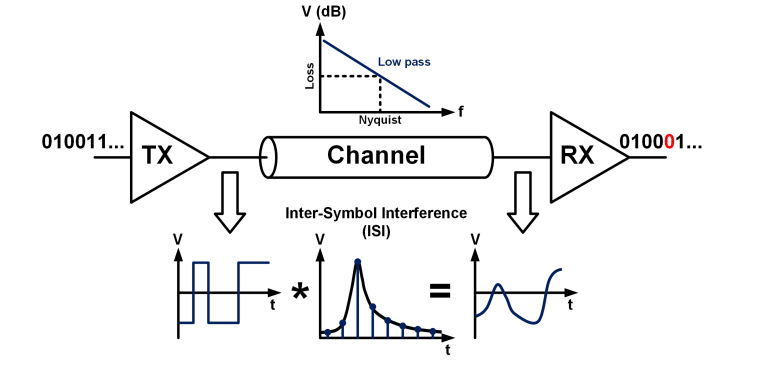
\includegraphics[width=12cm,height=6cm]{fig1.png}
	\caption{Block Diagram of a Simple Communication Channel [4]}
	\label{block_diag}
\end{figure*}

Eye diagrams provide a pictorial way to judge whether a channel/link is healthy. Eye diagrams are generated by overlapping unit intervals (UI) of the signal of interest in the time domain. Figure 1.2 shows examples of open and closed eye diagrams. When channel ISI and noise in the link system is much smaller than the actual data signal, we obtain an open eye diagram (Figure 1.2(a)) in which the eye has a vertical opening, eye height (E.H) and a horizontal opening, eye width (E.W). The dither around the data levels are due to residual ISI and noise. Figure 1.2(b) shows an example of a closed eye diagram. In such a system, ISI and noise overwhelm the transmitted data, therefore making the high and low data levels indistinguishable. For a given PAM scheme, there will be PAM-1 eyes in the eye diagram. \\

\begin{figure*}
	\centering
	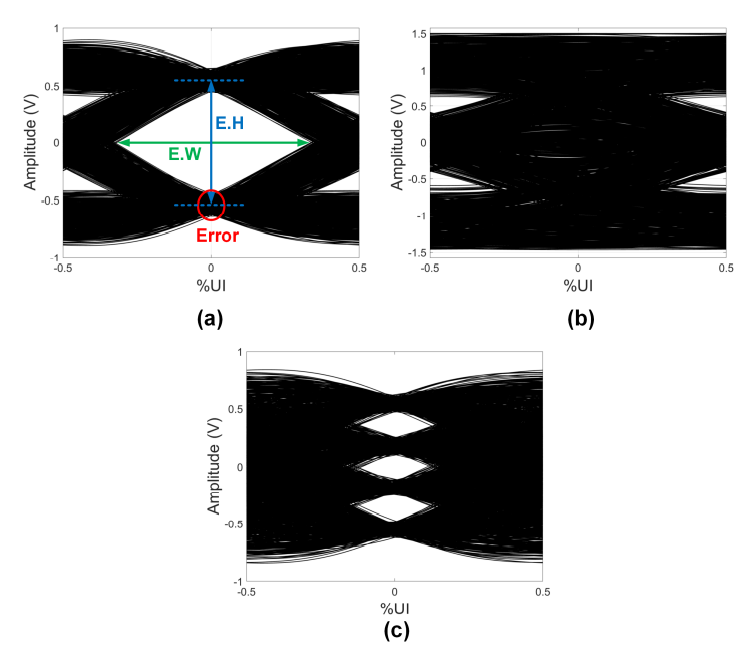
\includegraphics[width=12cm,height=8cm]{fig1_2.png}
	\caption{Examples of (a) an open eye diagram for PAM2, (b) a closed eye diagram
for PAM2 and (c) an open eye diagram for PAM4 [4]}
	\label{PAM_eye}
\end{figure*}

Bit error rate (BER) is the metric that ultimately quantifies a link's performance. As illustrated by the PAM2 example in Figure 1.3, the TX only sends voltages representing either a "0" or "1" in the probability domain. After channel ISI and circuit/environment noise are added, the receiver sees a signal whose probability density function (PDF) is a sum of two Gaussian-like peaks. The area under the curves' crossed-over portions gives the probability of a wrong bit decision, thus BER.\\

\begin{figure*}
	\centering
	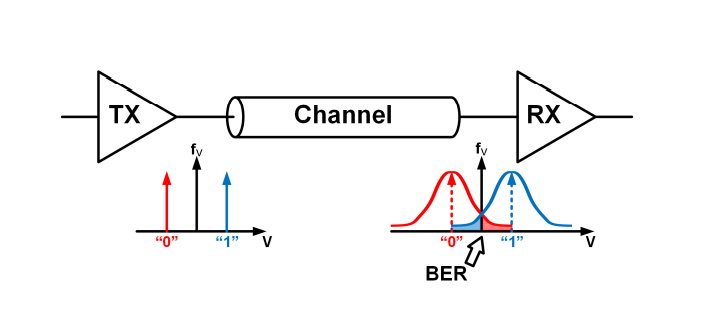
\includegraphics[width=12cm,height=6cm]{fig1_3.png}
	\caption{Bit error rate in wireline links [4]}
	\label{BER_links}
\end{figure*}

In order to compensate for ISI due to channel loss and meet the required BER specifications, different equalization techniques are used in link systems. Figure 1.4 shows conventional mixed-signal equalization blocks on both the TX and RX end [4]. The main cursor in a channel's pulse response is the signal of interest. Any ISI cursors before the main cursor are called pre-cursors. A feed-forward equalizer (FFE), which is typically implemented on the TX side, normally cancels pre-cursors. Any ISI cursors following the main cursor are considered post-cursors, which are often taken care of by the receiver with a continuous-time linear equalizer (CTLE) and decision feedback equalizer (DFE). The CTLE acts as high-pass filter to compensate for the channel's low-pass action. Due to the high-pass nature of CTLEs, any high frequency receiver input noise will be boosted similar to the actual signal. To avoid excessive noise amplification, DFEs pass the noise-less recovered bits through a finite impulse response (FIR) filter that matches the post-cursor portions of the channel to achieve ISI cancellation. The TX FFE can also provide some coarse equalization for post-cursors.

\begin{figure*}
	\centering
	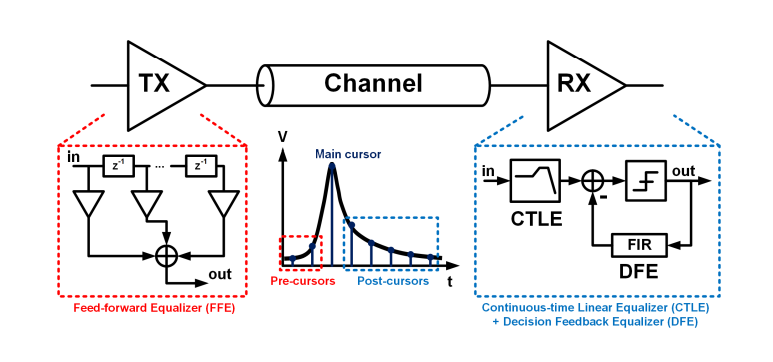
\includegraphics[width=12cm,height=6cm]{fig1_4.png}
	\caption{Equalization in conventional mixed-signal links [4]}
	\label{BER_links}
\end{figure*}


\section{Organization}
\rhead{Organization}
\begin{itemize}
	\item To understand the application space for ADCs	, we first review the 
basic concepts of high-speed link systems in Chapter 2.
	\item In Chapter 3, we look in detail, at the design of a sub-ADC including Sampling switch, StrongARM Latch, SAR Logic and the integration of these elements to form an SAR ADC.
	\item In Chapter 4, we take a look at the preliminary results that we have obtained in the due course of this work thus far.
	\item In Chapter 5, the work to be done in the future will be discussed followed by conclusions.
	\item In Chapter 6, various references have been cited.
\end{itemize}

\newpage


  \newpage 
%  %\newpage\null\newpage
  
\chapter{An Overview of High-Speed Link Systems}
\graphicspath{{An Overview of High-Speed Link Systems/Vector/}{An Overview of High-Speed Link Systems/}}

A typical high-speed link system consists of 3 basic components: a 
serializing transmitter, a communication channel, and a deserializing receiver, as 
shown on the block diagram in Figure 2.1.

\begin{figure*}
	\centering
	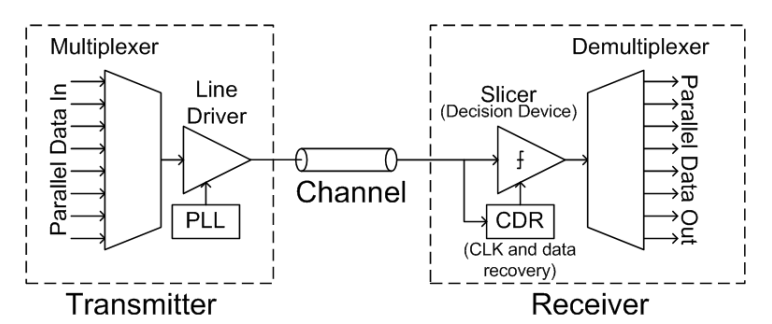
\includegraphics[width=14cm,height=6cm]{fig2_1.png}
	\caption{Block diagram of a high-speed link [5]}
	\label{high_sp_bl_diag}
\end{figure*}

The transmitter usually includes a multiplexer that converts parallel 
data into serial stream, a line driver that send data bits through the physical channel, 
and a clock source, usually implemented as a phase-locked loop (PLL). \\
The receiver decides which discrete digital value has most likely been 
transmitted. The decision device is usually referred to as slicer or comparator. Then 
the serial data stream is usually demultiplexed into parallel word, more naturally 
suited for data processing. If no explicit clock signal is sent along with the data, a clock and data recovery (CDR) block is needed to derive the timing information 
from data transitions.\\

A convenient way of describing a channel is by the pulse response of the channel. A pulse response of the channel is its output resulting from 
an isolated single-bit pulse (…0001000…) at its input. A general low-pass nature of 
most channels suggests that they cannot instantaneously respond to infinitely sharp 
edges of a pulse, delaying and dispersing it, as shown in Figure 2.2. When such pulse 
response is sampled at bit times, the largest sample is called the cursor; the samples 
before the cursor are called pre-cursors, and the samples after the cursors are called post-cursors. Pre-cursors interfere with previously sent bits, while post-cursors 
interfere with the following bits. To cancel such inter-symbol interference, most 
modern links use equalization. An equalizer provides an inverse channel response 
such that the overall frequency response is flat over the bandwidth of interest.

\begin{figure*}[h]
	\centering
	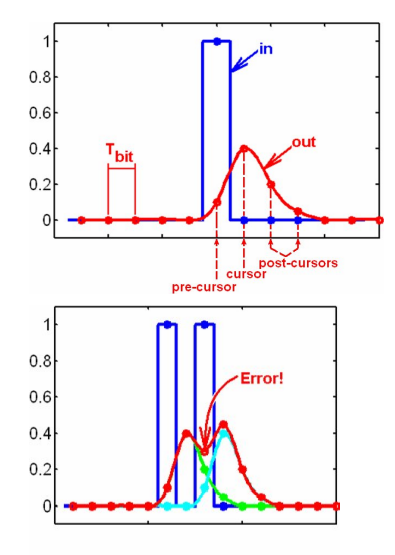
\includegraphics[width=6cm,height=10cm]{fig2_2.png}
	\caption{Pulse dispersion and inter-symbol interference [5]}
	\label{ISI}
\end{figure*}

%%%%%%%%%%%%%%%%%
%%%%%%%%%%%%%%%%%%
%%%%%% Chapter 2 Section 1
%%%%%%%%%%%%%%%%%
%%%%%%%%%%%%%%%%%%
\section{Linear Equalization}
Equalization is an important application space for digital-to-analog and 
analog-to-digital converters. Equalizer implementations fall into 3 general categories: 
analog, semi-digital, and digital. As we shall see, this classification is somewhat 
oversimplified, because most "analog" equalizers incorporate some digital adjustment, 
while all "digital" equalizers require ADCs and DACs to interface digital processors with analog channels. In fact, most equalizers operate on both analog and digital 
signals, so ADCs and DACs are needed to perform the conversion between the two 
domains. It is mainly equalizers that drive the development of data converters in high-speed links. To understand how ADCs can be optimized for this purpose, let us 
describe a few most common equalization techniques used in high-speed links.

\section{Digital Feedback Equalization}
\rhead{Digital Feedback Equalization}

All linear equalizers suffer from another problem. Ideally, an equalizer 
placed at the transmitter would boost a signal at high frequencies leaving low-frequency content intact. However, due to limited voltage swing of the channel driver, 
the filter is forced to attenuate lower frequencies rather than amplify higher 
frequencies, reducing the total signal energy and, thus, the signal-to-noise ratio (SNR). 
On the other hand, an equalizer placed at the receiver amplifies high-frequency noise 
along with the signal, again degrading the SNR.\\

To circumvent such noise amplification problem, non-linear equalizers 
can be used. The simplest, efficient, and thus most common non-linear equalizer used 
in high-speed link receivers is a decision-feedback equalizer (DFE), depicted in 
Figure 2.3 for a 4-tap example. Assuming that the 4 previous bits were detected 
correctly, DFE subtracts their influence from the currently received analog input 
voltage, thus cancelling their post-cursor ISI. Note that DFE cannot cancel pre-cursor 
ISI, because the cursor bit has not been sliced yet.

\begin{figure*}[h]
	\centering
	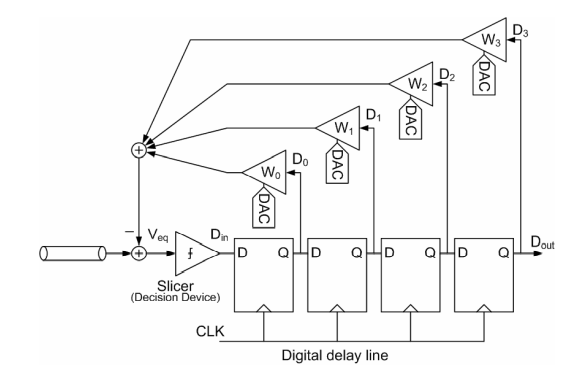
\includegraphics[width=12cm,height=8cm]{fig2_3.png}
	\caption{Decision-feedback equalizer on the receiver side
[5]}
	\label{DFE}
\end{figure*}

Nevertheless, DFE is very useful, because due to its non-linear nature 
(it contains a comparator), it does not amplify high-frequency noise from the channel. 
It is susceptible to error propagation, however, meaning that if a bit has been 
incorrectly detected, its ISI will not be corrected properly, leading to error propagating 
to the current bit. While this may cause chains of errors in low-SNR channels (like 
wireless), such error propagation is much less probable in higher-reliability short-reach copper links.


\section{Digital Equalizer Implementations}
\rhead{Digital Equalizer Implementations}

Implementing a filter in digital domain allows one to compute filtering 
results with higher resolution in digital domain and then round them off only once to 
the closest data converter level. This is in contrast with semi-digital implementation, 
where the value of each tap is rounded off, leading to accumulation of rounding errors. 
This problem is illustrated in Figure 2.4. Only three taps are shown for simplicity, but 
one can imagine the problem only getting worse for more taps. 
To understand this issue more fully, we can view the operation of the 
filter as a function of data bits as moving along a tree. The "root" of the tree is output 
for no filter taps. For one single tap, depending whether the previous data bit was 0 or 
1, the filter output branches to either (–W0) or W0. If the filter has two taps, depending 
on whether data bits were 00, 01, 10, or 11, there are four possibilities for the filter 
output: (-W1,-W0), (-W1,+W0), (+W1,-W0), and (+W1,+W0). For 3 taps, there are 8 possible 
outputs, and for $N_{taps} \  taps \,–\,
2^{N_{taps}}$ . Figure 2.4(a) shows the tree without any 
quantization. Figure 2.4(b) illustrates how quantization of each individual tap weight 
leads to error accumulation. Finally, Figure 2.4(c) shows that computing filter output 
with higher precision in digital domain and then rounding solves the error 
accumulation problem.\\

\begin{figure*}[h]
	\centering
	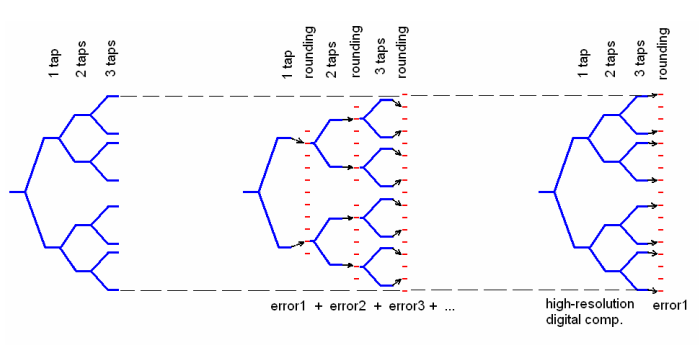
\includegraphics[width=12cm,height=8cm]{fig2_4.png}
	\caption{FIR filter output as a function of input bits (a) without any quantization, (b) 
with each tap weight Wi quantized separately, and (c) with filter output computed 
digitally with high resolution and then rounded off to the closest available data 
converter level [5]}
	\label{dig_fil_err_acc}
\end{figure*}

Unfortunately, implementing a digital filter at high speed and with high 
resolution is also problematic. Thus, instead of performing digital computations on-the-fly, look-up tables (LUTs) can be used, as demonstrated by B. Casper, et. al. in 
[6] for transmit equalization.



\section{ADC for Receiver Equalization}
\rhead{ADC for Receiver Equalization}

Apart from digital filters, the digital transmit equalizer requires a baud-rate 
DAC, while the digital receive equalizer requires a baud-rate ADC. As baud rates of 
modern links extend well into Gbps range, both DACs and ADCs operating at such 
rates are large research topics in themselves. In this work, we focus only on designing 
high-speed ADCs for the link receivers. The complexity, and even feasibility, of this 
task as well as the choice of the ADC topology depend on system requirements for the 
ADC. While the baud rate of the link determines the sampling rate of the ADC, its 
resolution is defined by two considerations. \\
First, the LSB size must be small enough so that it does not noticeably degrade 
the noise margin of the link, defined by half a signal swing minus all bounded error 
sources. Equalization normally removes the precursor and postcursor ISI, leaving only 
the main cursor as a signal to be detected and reducing the useful signal swing by the 
sum of magnitudes of all pre- and post-cursors. On top of this attenuation, the bounded 
error sources include unequalized ISI, reflections, and crosstalk. The ADC 
quantization error becomes an additional bounded error source, and thus should be 
kept to a small fraction $\alpha$ of the main cursor. The value of $\alpha$ should be typically less 
than 10-20%. 
\\
Second, the ADC range must cover the entire swing of the receiver input, 
including the worst-case effects from the pre- and post-cursor ISI (unless they have 
been cancelled by the transmit equalizer). The worst-case signal swing is equal to the 
sum of magnitudes of all taps in a pulse response (pre- and post-cursors plus the cursor 
itself).\\
Given these two considerations, the number of ADC levels ( $$ N_{levels}=2^{N_{bits}} $$ ) 
should be approximately: 

$$ N_{levels}=2^{N_{bits}}=\sum_{i=-\infty}^{\infty} |P_i|/{\alpha.P_0} $$\\

where $P_{i}$ is the $i{th}$ tap in a channel pulse response, with i < 0 for pre-cursors, i > 0 for post-cursors and i = 0 for the main-cursor. $\alpha$ is the fraction of equalized signal 
amplitude allocated to quantization error of the ADC. Taking $\alpha$ = 10\% and pulse 
response shown in Figure 2.2 as an example, we obtain $N{levels} = 20 \ and\  N{bits} = 4.3$. As it 
turns out, for most typical backplane channels, N{bits} of 4-5 bits is required. Thus, for 
this work, we will target a resolution of 6-7 bits.



  \newpage
%  %\newpage\null\newpage
  
\chapter{Sub-ADC Design}
\graphicspath{{Sub-ADC Design/Vector/}{Sub-ADC Design/}}

Figure 3.1 shows the common ADC 
topologies used in these serial links, 
which include flash, binary/multibit 
search, and successive approximation 
register (SAR). Flash ADCs employ 
comparators at each reference level, 
with a 6-b flash ADC requiring 63 comparators that simultaneously evaluate 
over a single cycle. This allows for very 
high-speed operation with relatively 
low time-interleave factors between 
four and eight. The main downside is the large comparator count, although 
rectifying architectures can reduce 
this. Overall, flash ADCs are a reasonable choice for PAM2, but the resolution is a bit low for PAM4.\\

\begin{figure*}
	\centering
	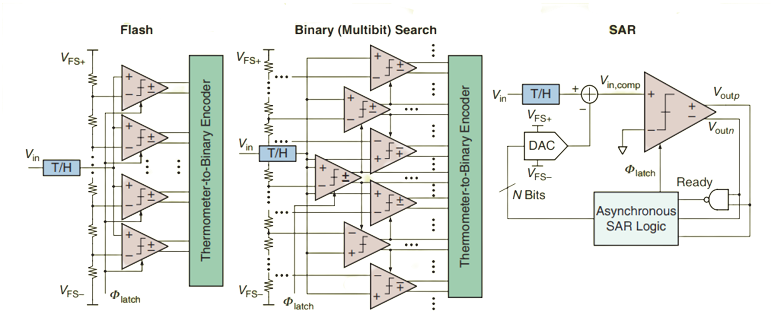
\includegraphics[width=12cm,height=6cm]{fig3_1.png}
	\caption{The common ADC topologies used in serial link receivers. [7]}
	\label{adc_topo}
\end{figure*}

Binary or multi-bit search ADCs 
combine desirable properties of flash 
and SAR ADCs. While conventional 
binary search ADCs have the same 
number of comparators as a flash 
ADC, the architecture employs a binary search algorithm with the most 
significant bit (MSB) comparator's output deciding which MSB-1 comparator is clocked, and so on. This results 
in only the necessary comparators 
evaluating, or six in a 6-b converter. 
The binary search ADC avoids the digital-to-analog converter (DAC) settling 
and logic delay present in SARs but is 
slower than a flash due to the serial 
comparator evaluation. Overall, this 
is also a good choice for PAM-2 applications, but the area is often high for 
PAM-4 applications.\\
An SAR ADC employs a binary search 
conversion over multiple clock cycles. 
The simplest implementations require 
only one comparator per unit ADC, 
whose decision adjusts a reference DAC 
to make the full signal quantization in a 
successive approximation manner, with 
a 6-b converter clocking the comparator 
six times. This results in a slower unit 
ADC relative to flash or binary search, 
with high-speed converters using higher 
interleave factors of 32–128. 
This is an excellent choice for 6–8-b resolution to support both PAM-2 and PAM-4, 
and it is the dominant architecture for 
PAM-4 ADC-based receivers. Given this, 
the next section provides an overview of key ADC circuits in the context of a time-interleaved SAR ADC. Note that many of 
the circuit concepts are also relevant to 
other ADC topologies.

\begin{figure*}[h]
	\centering
	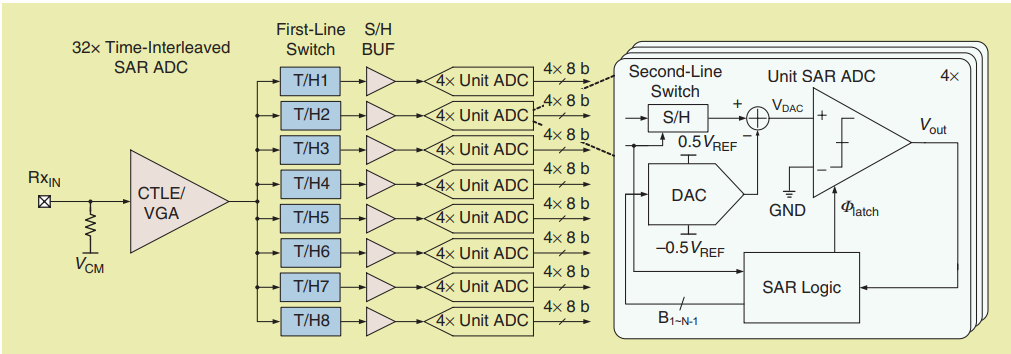
\includegraphics[width=10cm,height=6cm]{fig3_2.png}
	\caption{A 32-way time-interleaved SAR ADC. GND: ground; S/H BUF: sample/hold buffer. [7]}
	\label{TI-ADC}
\end{figure*}

%%%%%%%%%%%%%%%%%
%%%%%%%%%%%%%%%%%%
%%%%%% Chapter 3 Section 1
%%%%%%%%%%%%%%%%%
%%%%%%%%%%%%%%%%%%
\section{Sampling Switch}

The input T/H circuit must track 
and sample/hold the full-bandwidth 
input signal for further sampling by 
the unit ADCs. Due to this high-bandwidth requirement, many high-speed 
ADCs employ a bootstrapped T/H 
switch [11]. The collection of transistors and the offset storage capacitor 
shown in Figure 5 produce a signal independent overdrive on the main 
sampling switch to keep the tracking bandwidth constant. When the 
clock is low and the switch is off, the 
capacitor is precharged to VDD. One 
terminal of the capacitor is then connected to the input when the clock 
goes high, forcing the other terminal 
to VDD above it, which should result 
in a signal-independent VDD overdrive on the switch when it is on. This 
results in an improvement in signal-to-noise-and-distortion ratio (SNDR), 
particularly at high frequencies.

\begin{figure*}[h]
	\centering
	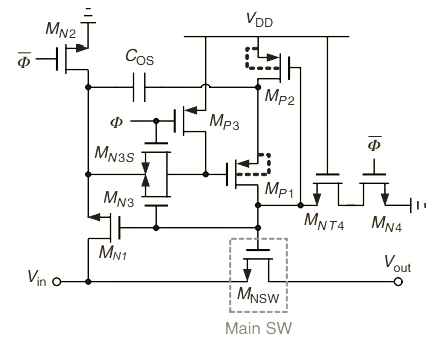
\includegraphics[width=10cm,height=7cm]{fig3_3.png}
	\caption{Bootstrapped T/H [7]}
	\label{TI-ADC}
\end{figure*}

After the second-line switch, the 
unit ADC consists of the capacitive 
reference DAC, the comparator, and 
SAR logic. The DAC generates residue 
signals for each bit conversion by 
subtracting a binary weighted reference from the sampled input signal. 
This is done via charge sharing in a 
capacitive DAC, with a typical $65\,nm$ 
CMOS implementation.



\section{StrongARM Latch}
\rhead{StrongARM Latch}
\label{StrongARM Latch}


The comparator is a sense amplifier that is desgined by using a StrongARM Latch topology. The StrongARM latch topology finds 
wide usage as a sense amplifier, 
a comparator, or simply a robust 
latch with high sensitivity. The term 
“StrongARM” commemorates the use 
of this circuit in Digital Equipment 
Corporation’s StrongARM microprocessor, but the basic structure was 
originally introduced by Toshiba’s 
Kobayashi. The StrongARM 
latch has become popular for three 
reasons: 
\begin{enumerate}[1.]
	\item it consumes zero static power
	\item it directly produces rail-to-rail outputs
	\item its input-referred offset arises from primarily one differential pair.
\end{enumerate}

\begin{figure*}[h]
	\centering
	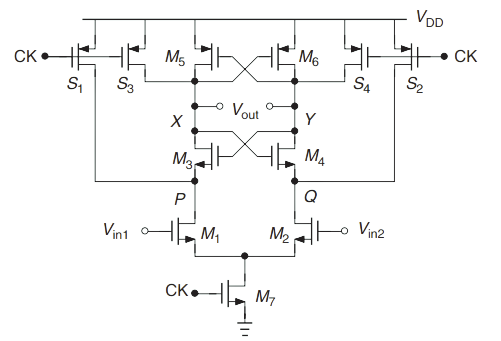
\includegraphics[width=10cm,height=6cm]{fig3_4.png}
	\caption{Modified StrongARM Latch [7]}
	\label{SAL}
\end{figure*}

The comparator makes a decision 
on the DAC signal to generate the output bits that serve as the binary search 
codes for the SAR logic that controls 
the DAC. Noise 
and offset considerations generally set 
the minimum comparator size. However, the brute-force design of a comparator for a given offset performance 
leads to excessive power and area in 
modern CMOS processes.

\newpage
\section{SAR Logic}
\rhead{SAR Logic}

Finally, the SAR logic generates both 
the comparator clock and the DAC control signals based on the comparator 
output. A conventional synchronous 
SAR ADC uses logic that generates an 
internal clock operating at N + 1 times 
the unit ADC sampling frequency to 
allow for one tracking cycle and N-bit 
conversion cycles. However, given 
metastability considerations, each cycle should be timed to satisfy the worst-case comparator input that will occur 
only once in the multi-bit conversion.
  \newpage
%  %\newpage\null\newpage
  
\chapter{Preliminary Results}
\graphicspath{{Preliminary Results/Vector/}{Preliminary Results/}}

The proposed SAR ADC architecture is being studied, researched, and simulated. So far, the bootstrapped T/H switch, and the StrongARM Latch have been simulated in Cadence Virtuoso tool. The channel has also been statistically modelled by including the effect of ADC's quantization noise in a SerDes link using MATLAB. The results are following sections.

%%%%%%%%%%%%%%%%%
%%%%%%%%%%%%%%%%%%
%%%%%% Chapter 4 Section 1
%%%%%%%%%%%%%%%%%
%%%%%%%%%%%%%%%%%%
\section{Time Domain Analysis of SerDes Link}

A RPBS sequence was generated and passed through an AWGN channel in a SerDes wireline channel. The eye diagram of the channel response was plotted as shown in Figure 4.1. \\

\begin{figure*}[h]
	\centering
	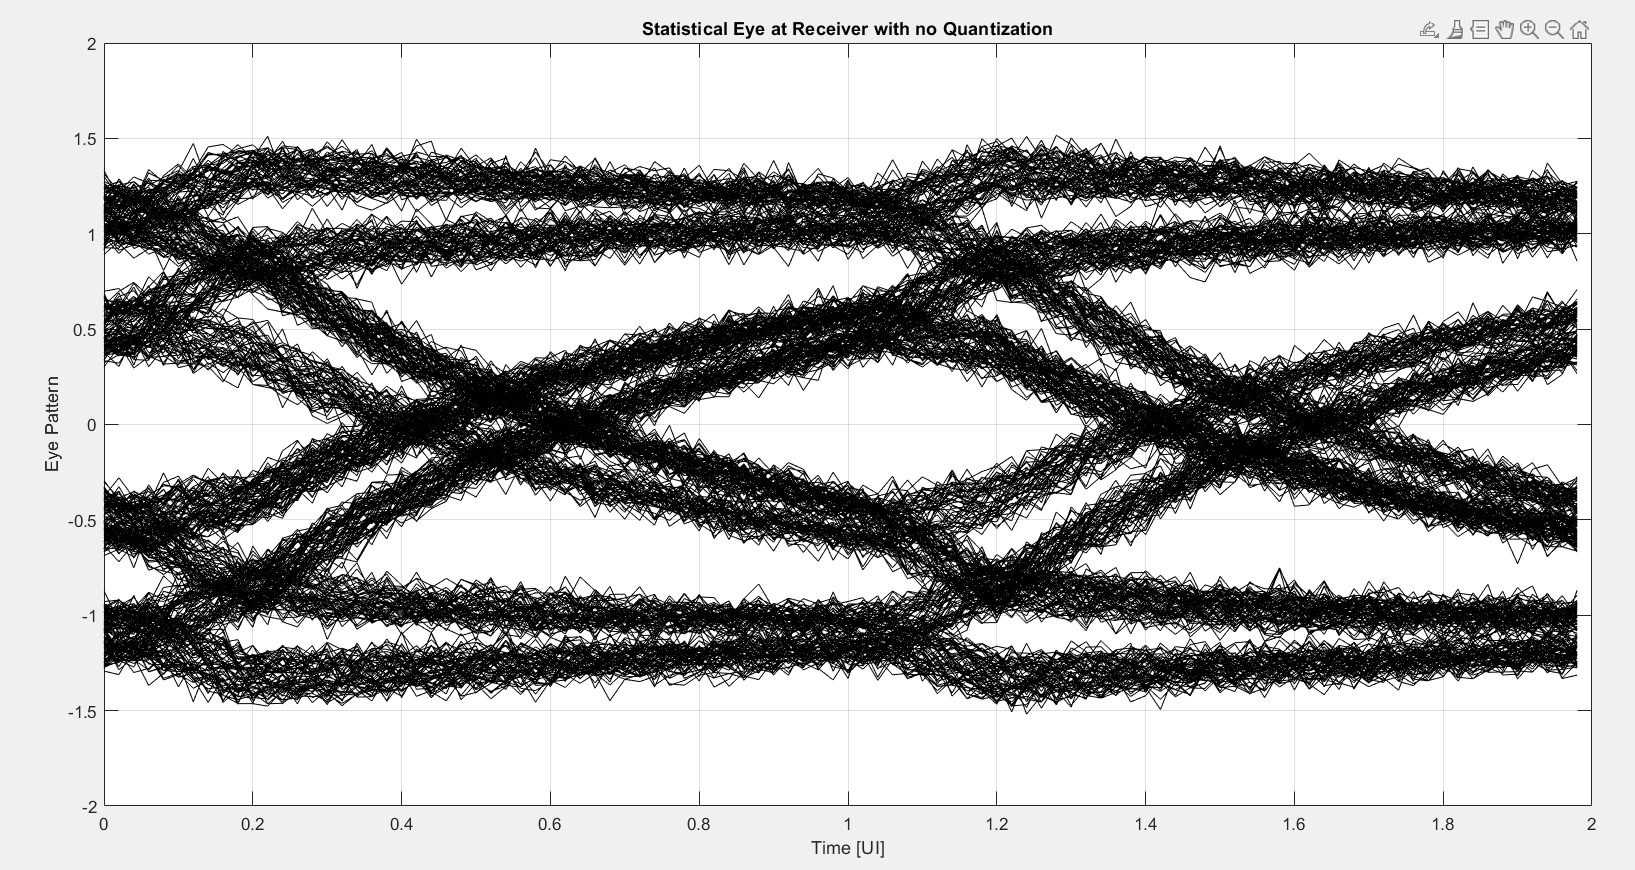
\includegraphics[width=12cm,height=6cm]{fig4_1.png}
	\caption{Statistical Eye with no Quantization}
	\label{eye_wo_q}
\end{figure*}

Next, quantization was added to the channel response in order to see the effect of including an ADC in the receiver. The waveforms clearly  shows that an open eye can be achieved with a quantization of about 5-6 bits and nothing lower than that. The eye diagrams for quantization with 8, 5, and 3 bits have been plotted in Figure 4.2 to understand this phenomena.

\begin{figure*}[h]
	\centering
	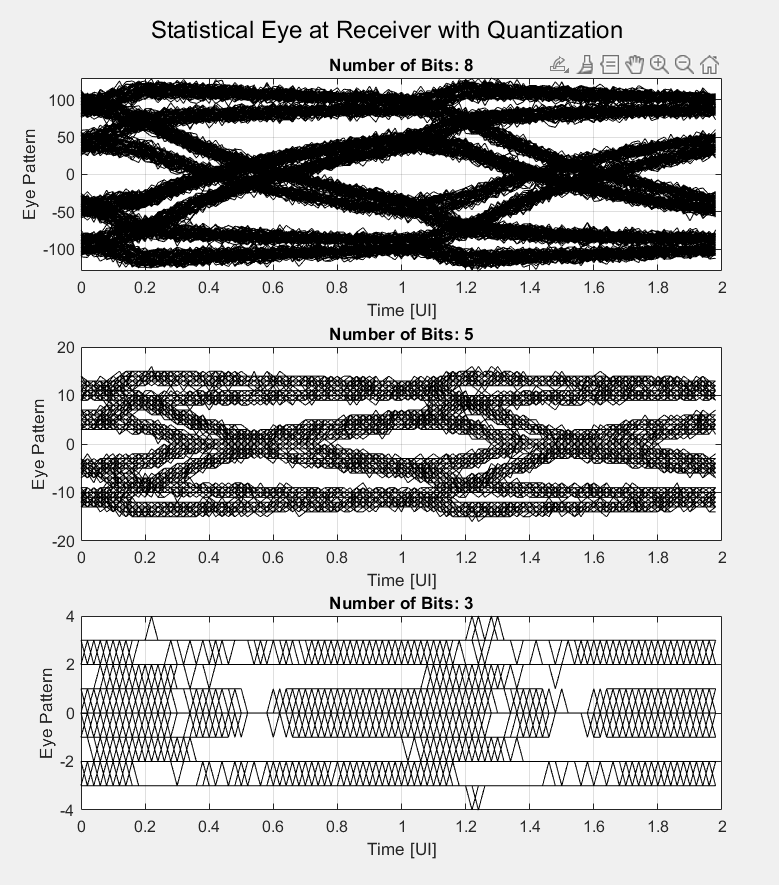
\includegraphics[width=12cm,height=12cm]{fig4_2.png}
	\caption{Statistical Eye with Quantization}
	\label{eye_w_q}
\end{figure*}


\section{Design of Sub-ADC}
\rhead{Design of Sub-ADC}
\label{Design of Sub-ADC}

\subsection{Bootstrapped switch}

A simple bootstrapped switch has been designed and simulated using the Cadence Virtuoso tool with $USMC\; 65\,nm$ PDK. The sampling frequency was chosen to be \textbf{$1\: GHz$} and the message signal frequency was chosen to be \textbf{$125\: MHz$}. The resulting waveform can be seen in the Figure 4.3. Very little non-idealities and non-linearities can be observed which are negligible.

\begin{figure*}[h]
	\centering
	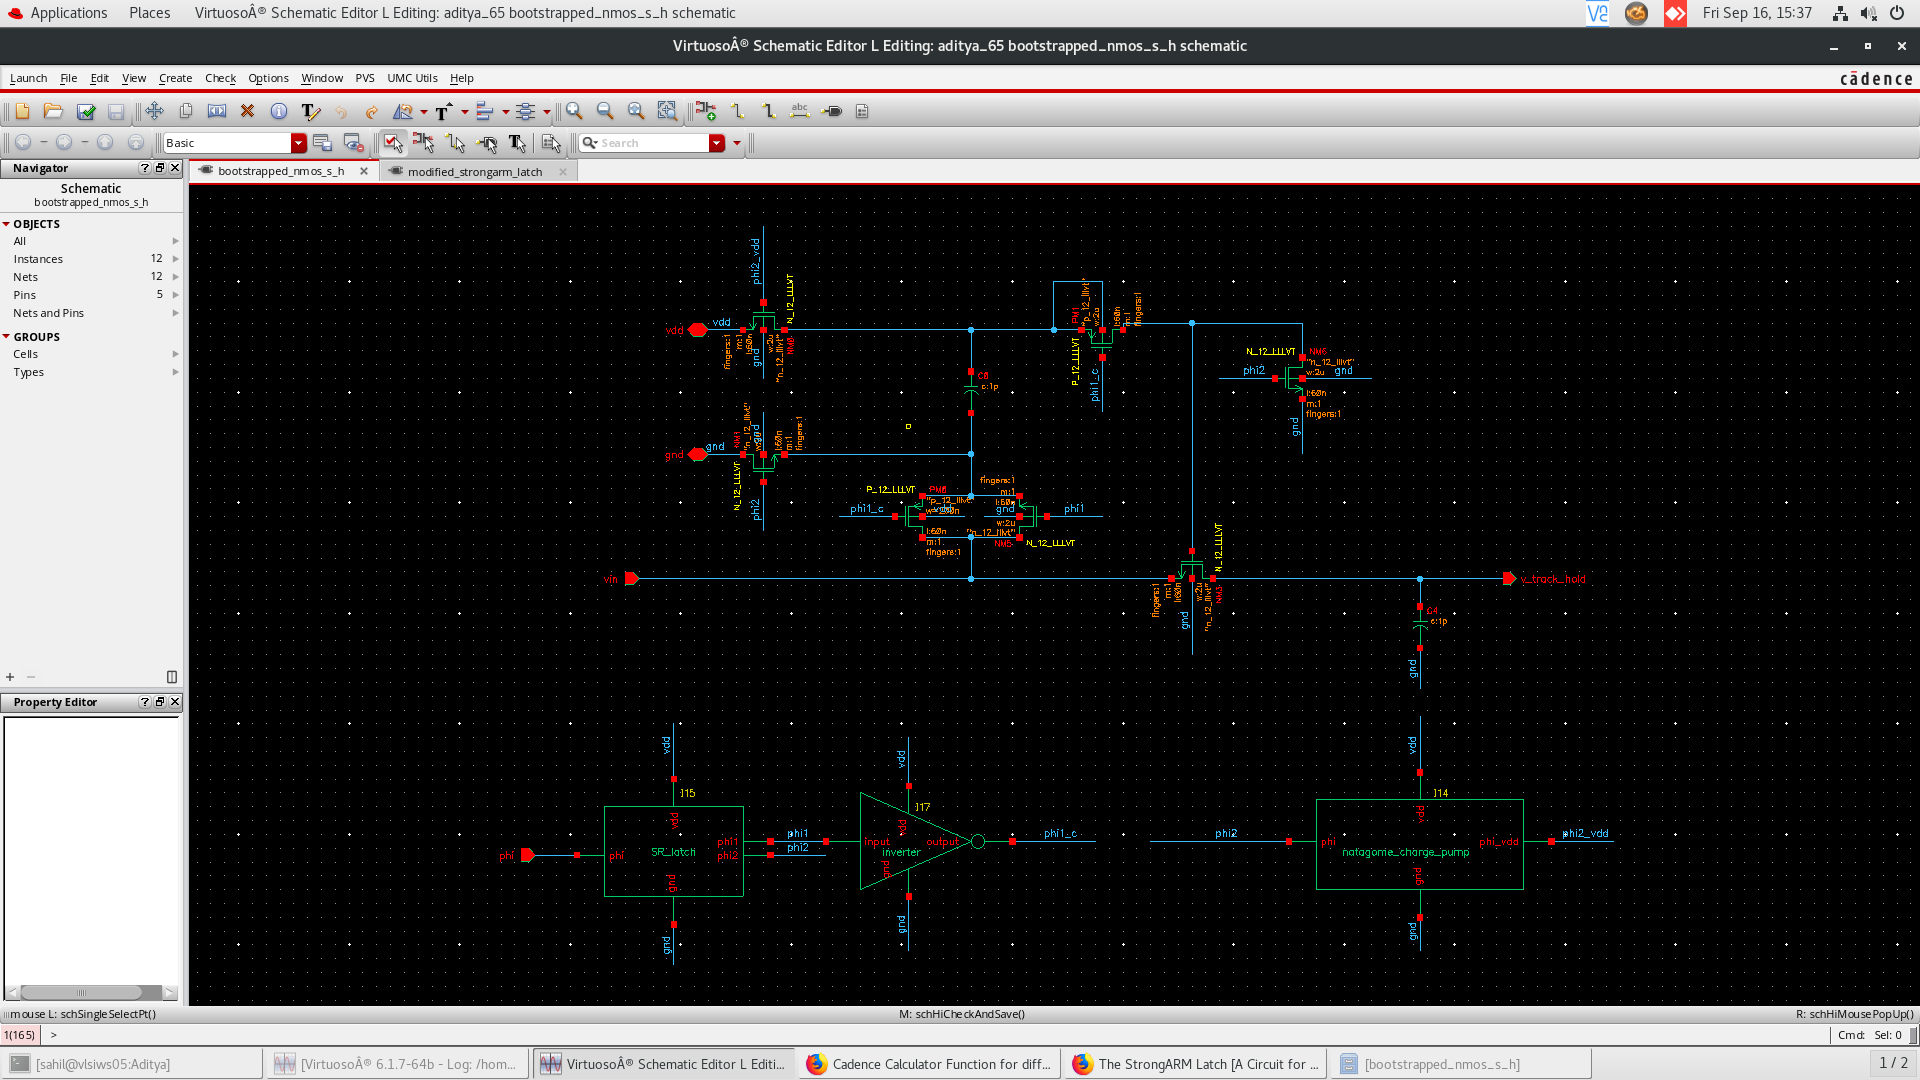
\includegraphics[width=16cm,height=8cm]{fig4_3.png}
	\caption{Bootstrapped Track and Hold Circuit Schematic}
	\label{t_h_ckt}
\end{figure*}

\begin{figure*}[h]
	\centering
	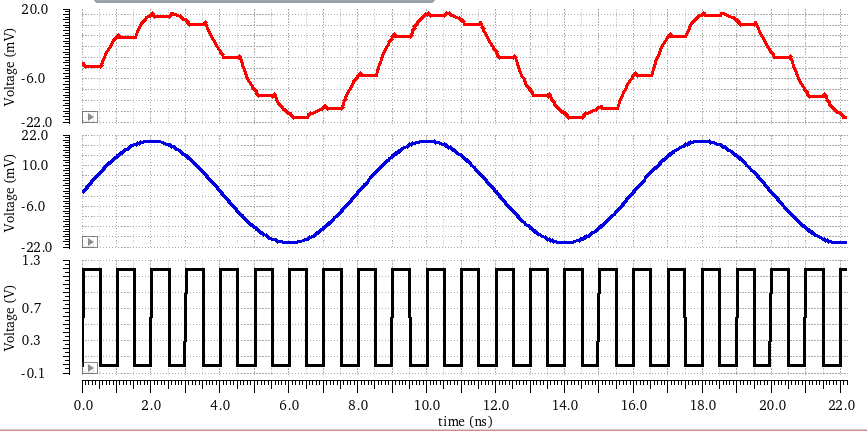
\includegraphics[width=16cm,height=8cm]{fig4_4.png}
	\caption{Bootstrapped Track and Hold Waveform}
	\label{t_h_waveform}
\end{figure*}

\subsection{StrongARM Latch}

A StrongARM Latch has also been simulated using Cadence Virtuoso tool in $USMC\! 65 \, nm$ PDK. The \textbf{Clock} was a pulse with a period of \textbf{1 GHz}. The input \textbf{$V_{in1}$} was \textbf{grounded}, whereas the input \textbf{$V_{in2}$} was connected to \textbf{$V_{DD}$}. The output clearly shows \textbf{$V_{x}$} reaches an output voltage of \textbf{$V_{DD}$}, while \textbf{$V_{y}$} settles to 0 voltage after a while within the clock cycle. 

\begin{figure*}[h]
	\centering
	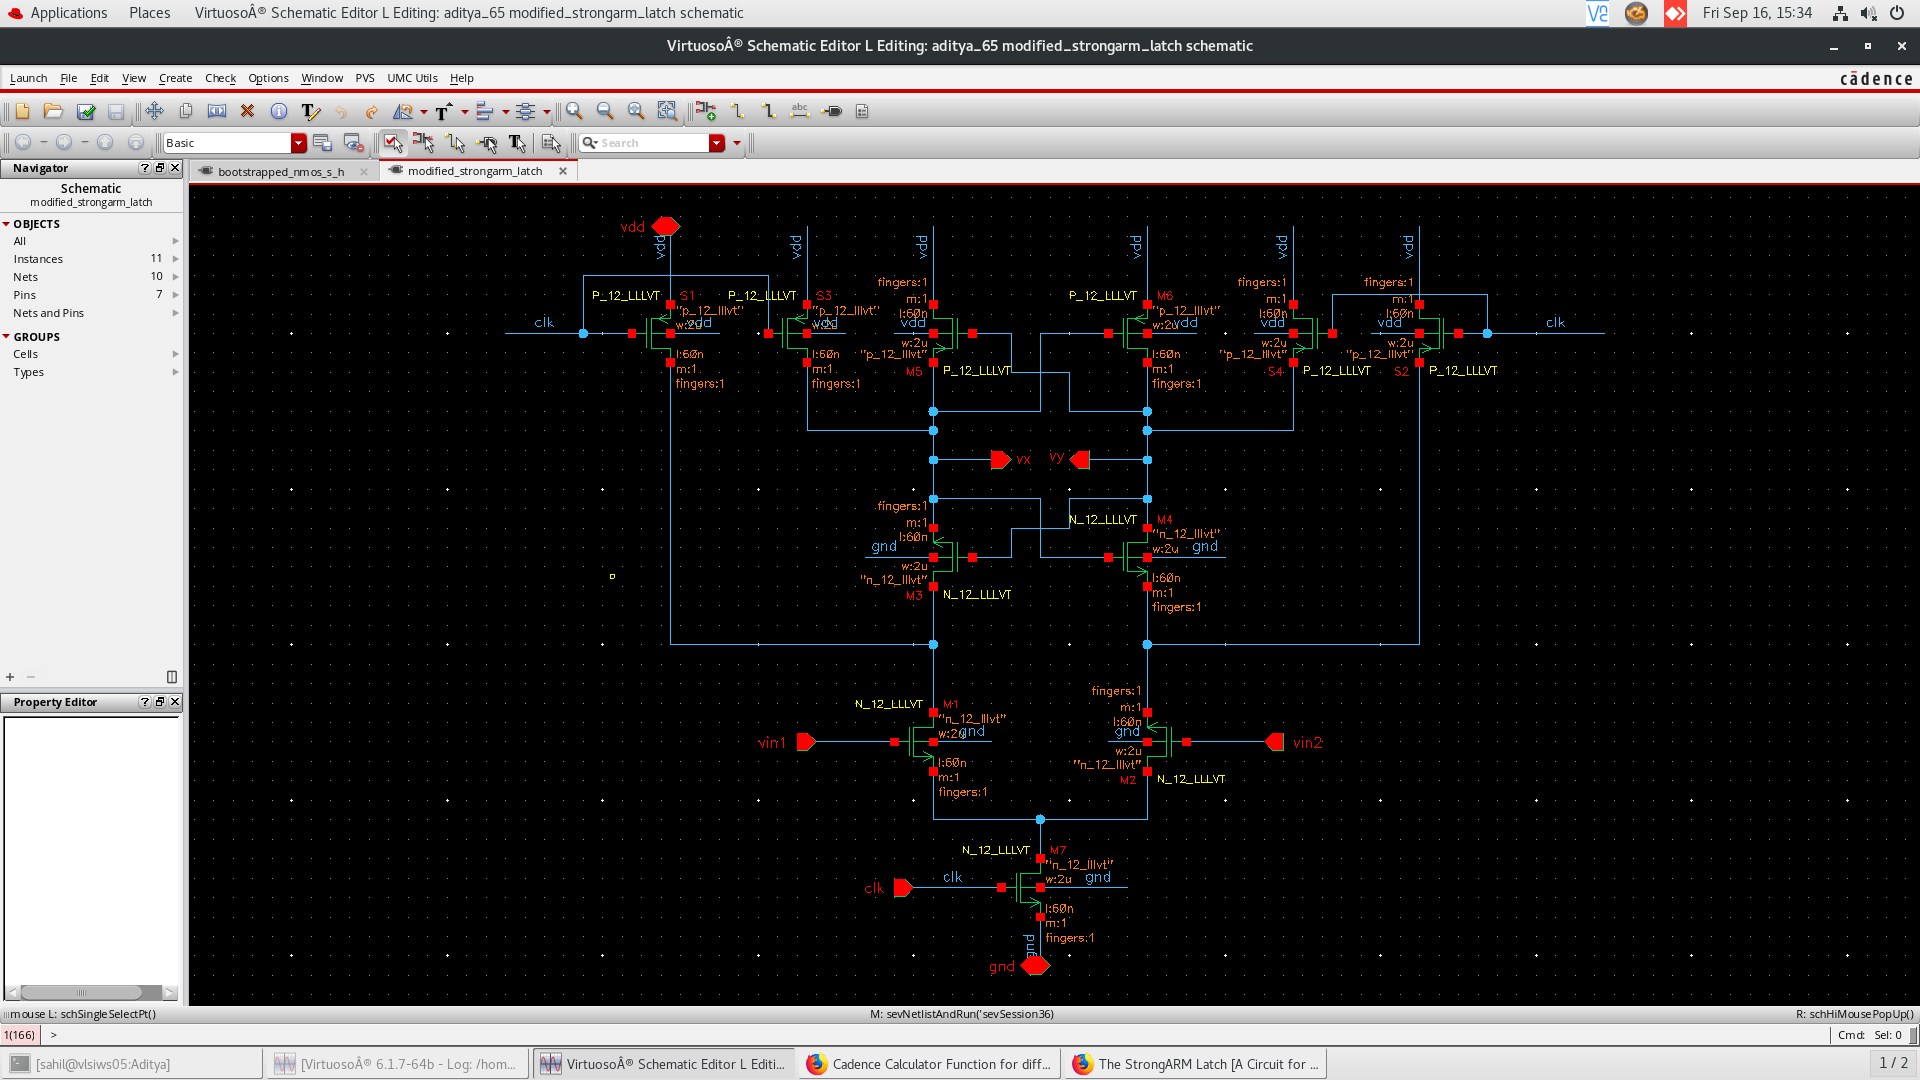
\includegraphics[width=16cm,height=8cm]{fig4_5.png}
	\caption{StrongARM Latch Circuit Schematic}
	\label{comp_ckt}
\end{figure*}

\begin{figure*}[h]
	\centering
	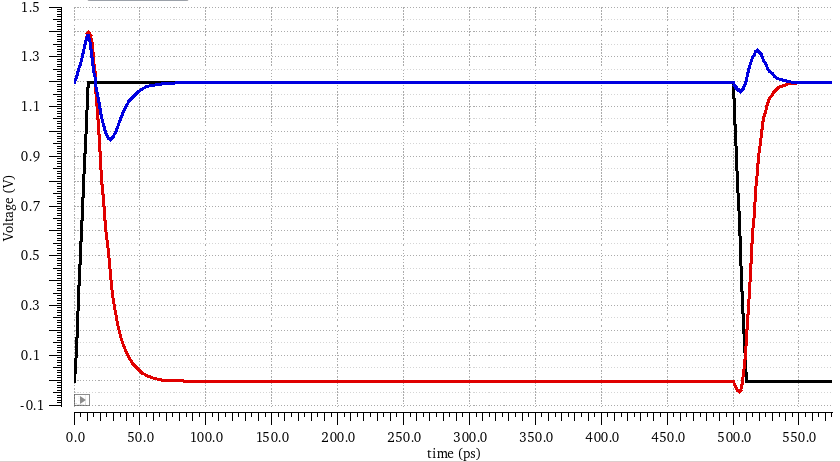
\includegraphics[width=16cm,height=8cm]{fig4_6.png}
	\caption{StrongARM Latch Output Waveform}
	\label{comp_waveform}
\end{figure*}

Another latch circuit has also been designed by clocking the differential pair through the cross-coupled NMOS pair in order to have a low kick-back current through the circuit when the circuit is in idle state. Its results can be seen in Figures 4.7-8. We can see that in the case of low kick-back circuit, the output voltages have more controlled peaks and peak only upto $1.3\,V$, whereas in the earlier case, the output voltages (\textbf{$V_{x}\: and \: V_{y}$}) peaked upto $1.4\,V$.

\begin{figure*}[h]
	\centering
	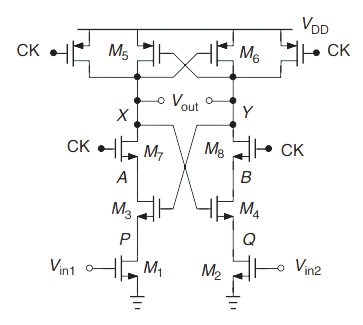
\includegraphics[width=12cm,height=8cm]{fig4_7.png}
	\caption{An alternative topology for lower kick-back noise [7]}
	\label{comp_lk_ckt}
\end{figure*}

\begin{figure*}[h]
	\centering
	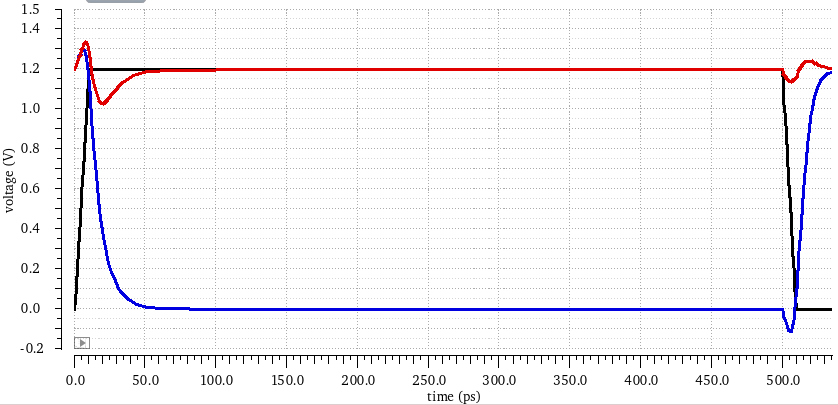
\includegraphics[width=16cm,height=8cm]{fig4_8.png}
	\caption{StrongARM Latch Low kick-back Output Waveform}
	\label{comp_lk_waveform}
\end{figure*}
\newpage
  \newpage
%  %\newpage\null\newpage
  
\chapter{Conclusions and Future Work}
\graphicspath{{Conclusions and Future Work/Vector/}{Conclusions and Future Work/}}
%%%%%%%%%%%%%%%%%
%%%%%%%%%%%%%%%%%%
%%%%%% Chapter 5 Section 1
%%%%%%%%%%%%%%%%%
%%%%%%%%%%%%%%%%%%
\section{Future Work to be Done}

So far, the track and hold switch and slicer of the unit ADC have been designed and simulated using Cadence Virtuoso tool USMC $65\,nm$ technology package. By the end of this semester, the complete design and simulation of the ADC is expected to be completed. \\
In the second part of my thesis, further enhancements will be made to the designed sub-ADC and will be made useful for integrating the ADC-based Receiver with SerDes links in real life.



\section{Conclusions}
\rhead{Conclusions}
\label{Conclusions}

The results thus far obtained of the circuits designed were found to be satisfactory as approved by me supervisor Dr Nijwm Wary. Few circuits in this report have been directly attached as screen shots taken from Cadence Virtuoso. I hereby, claim no responsibility of those diagrams. In future reports, I will take care that all the circuits will be drawn by me and the plots will be redrawn.
  \newpage
%  %\newpage\null\newpage  
%\lhead{}
%\rhead{\footnotesize Appendix}
%\appendix
%\addcontentsline{toc}{chapter}{Appendix}
%
%%%%% Creating Appendix A
	\chapter{}
	\label{appendix0}
		\graphicspath{{Appendices/Vector/}{Appendices/}}
	%%% Lauricella's Hypergeometric Functions
	%%%%%
\section*{Title of Appendix}
%%%%%%%%%%%%%%%%%%%%%%%%%%%%%%%%%%% 
%%%%%%%%%%%% Complete System Diagram
%%%%%%%%%%%%%%%%%%%%%%%%%%%%%%%%%%%

xxxxxx xxxxxx xxxxxx xxxxxx xxxxxx xxxxxx xxxxxx xxxxxx xxxxxx xxxxxx xxxxxx xxxxxx xxxxxx xxxxxx xxxxxx xxxxxx xxxxxx xxxxxx xxxxxx xxxxxx xxxxxx xxxxxx xxxxxx xxxxxx xxxxxx xxxxxx xxxxxx xxxxxx xxxxxx xxxxxx xxxxxx xxxxxx xxxxxx xxxxxx xxxxxx xxxxxx xxxxxx xxxxxx xxxxxx xxxxxx xxxxxx xxxxxx xxxxxx xxxxxx.

\begin{align}
y=\alpha\,x+n
\end{align} 
%%\input{Appendices/appendix1}
%%\input{Appendices/appendix2}
%%\input{Appendices/appendix3}
%  \newpage
%  \singlespacing
%%   %\newpage\null\newpage
%\pagestyle{fancy}
%\fancyhf{}
%\rhead{\fancyplain{}{Publications}}
%\cfoot{\fancyplain{}{\thepage}}
%  \addcontentsline{toc}{chapter}{Publications}
%  	\chapter*{Publications}
	\graphicspath{{Publications/Vector/}{Publications/}}
	\noindent{\bf {Journal Publications}}
	\begin{enumerate}
		\item{ }
		\item{ }
		\item{ }
		
		
		
	\end{enumerate}
	\noindent{\bf{Conference Publication}}
	\begin{enumerate}
		\item 
		\item
		
	\end{enumerate}
%  \newpage
%\singlespacing
%\pagestyle{fancy}
%\fancyhf{}
%\rhead{\fancyplain{}{Bibliography}}
%\cfoot{\fancyplain{}{\thepage}}
%\addcontentsline{toc}{chapter}{Bibliography}
%\bibliographystyle{IEEEtran}
	\chapter{References}

\begin{enumerate} [1.] 
	\item  D. C. Daly, L. C. Fujino, and K. C. Smith. Through the Looking Glass - The 2018 Edition: Trends in Solid-State Circuits from the 65th ISSCC. IEEE Solid State Circuits Magazine, 10(1):30–46, winter 2018. ISSN 1943-0582. doi: 10. 1109/MSSC.2017.2771103.
	\item IEEE Standard for Ethernet Amendment 10: Media Access Control Parameters, Physical Layers, and Management Parameters for 200 Gb/s and 400 Gb/s Operation. IEEE Std. 802.3bs, 2017.
	\item Common Electrical I/O (CEI) - Electrical and Jitter Interoperability agreements for 6G+ bps, 11G+ bps, 25G+ bps I/O and 56G+ bps. OIF CEI 4.0, 2017.
	\item Kevin J. Zheng. SYSTEM-DRIVEN CIRCUIT DESIGN FOR ADC-BASED WIRELINE DATA LINKS. Thesis Ph.D. Stanford University 2018.
	\item Valentin Abramzon. ANALOG-TO-DIGITAL CONVERTERS FOR HIGH-SPEED LINKS. Thesis Ph.D. Stanford University 2008.
	\item H. Casper et. al., A 20Gb/s Transceiver. IOCE, pp 90-91.
	\item S. Palermo, S. Hoyos, S. Cai, S. Kiran and Y. Zhu, "Analog-to-Digital Converter-Based Serial Links: An Overview," in IEEE Solid-State Circuits Magazine, vol. 10, no. 3, pp. 35-47, Summer 2018, doi: 10.1109/MSSC.2018.2844603.
	


\end{enumerate}
	\newpage


\end{document}

